\documentclass{standalone}
%\documentclass[a4paper,10pt]{scrartcl}

\usepackage[utf8]{inputenc}
\usepackage{tikz}
\usetikzlibrary{fit}

\begin{document}

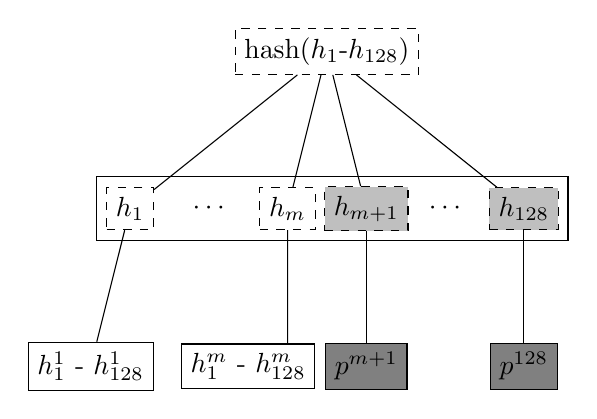
\begin{tikzpicture}
\node[draw,dashed] (root) at (3.5,3) {hash($h_1$-$h_{128}$)};
\node[draw,dashed] (h1) at (1,1) {$h_1$};
\node (dots1) at (2,1) {$\cdots$};
\node[draw,dashed] (h100) at (3,1) {$h_{m}$};
\node[draw,fill=lightgray,dashed] (h101) at (4,1) {$h_{m+1}$};
\node  (dots2) at (5,1) {$\cdots$};
\node[draw,fill=lightgray,dashed] (h128) at (6,1) {$h_{128}$};
\node[draw,fit=(h1) (dots1) (h100) (h101) (dots2) (h128)]{};
\draw (root) -- (h1);
\draw (root) -- (h100);
\draw (root) -- (h101);
\draw (root) -- (h128);
%
\node[draw] (g1) at (0.5,-1) {$h^1_1$ - $h^1_{128}$};
\node[draw] (g100) at (2.5,-1) {$h^{m}_1$ - $h^{m}_{128}$};
\node[draw,fill=gray] (p101) at (4,-1) {$p^{m+1}$};
\node[draw,fill=gray] (p128) at (6,-1) {$p^{128}$};
%
\draw (h1) -- (g1);
\draw (h100) -- (g100.30);
\draw (h101) -- (p101);
\draw (h128) -- (p128);

\end{tikzpicture}
\end{document}
